\documentclass[11pt,a4paper]{article} 
\usepackage[utf8]{inputenc}
\usepackage[ngerman]{babel}
\usepackage{amsmath}
\usepackage{amssymb}
\usepackage{geometry}
\usepackage{float}
\geometry{
  left=3cm,
  right=3cm,
  top=3cm,
  bottom=3cm,
  bindingoffset=0mm
}
\usepackage{graphicx}
\usepackage{xcolor}
\usepackage{mdframed}

\title{
	Modellierung einer Epidemie mittels eines zellulären Automaten
}

\begin{document}
\maketitle

\noindent
\textit{oder soll das Wort Corona bereits als zusätzlicher Eyecatcher in den Titel?}

\section{Einleitung}
Hier sicher etwas zu Corona aber mit einem \textbf{fetten} Hinweis, dass es keine wissenschaftliche Arbeit ist und vielmehr ein Erklärstück zu Differenzengleichungen und zellulären Automaten. \textit{Hier wäre ich sehr froh um etwas Hilfe aus der Kommunikationsabteilung ;-).}

\section{Das SIR-Modell}
Erklären was ein Differenzengleichungssystem ist (\(X_{k+1} = ... X_k ...\)).\\
Die drei Gruppen
\begin{itemize}
	\item \(S_k\): Gesunde Individuen (Susceptible)
	\item \(I_k\): Infizierte Individuen (Infected)
	\item \(R_k\): Immune Individuen (Resistant)
\end{itemize}
erklären und damit die Gleichungen
\begin{align*}
	S_{k+1} &= S_k - \alpha \cdot S_k \cdot I_k \\
	I_{k+1} &= I_k + \alpha \cdot S_k \cdot I_k - \beta \cdot I_k \\
	R_{k+1} &= R_k + \beta \cdot I_k
\end{align*}
herleiten. Dabei die Modellparameter
\begin{itemize}
	\item Infektionsrate \(\alpha\)
	\item Genesungsrate \(\beta\)
\end{itemize}
erklären.

\subsection{Die Basisreproduktionszahl \(R_0\)}
\label{sec:basis}
Die Basisreproduktionszahl gibt an wieviele Individuen ein Infizierter ansteckt, wenn noch kein Anteil der Population immun gegen die Krankheit ist.\\
\begin{mdframed}[backgroundcolor=gray!10,linewidth=0pt]
« R0 can be expressed as R0 = kbD, where k is the number of contacts each infectious individual has per unit time, b is the probability of transmission per contact between an infectious case and a susceptible person, and D is the mean duration of infectiousness. »\\
Quelle: Lipsitch, Marc; Cohen, Ted; Cooper, Ben; Robins, James M.; Ma, Stefan; James, Lyn; Gopalakrishna, Gowri; Chew, Suok Kai; Tan, Chorh Chuan; Samore, Matthew H.; Fisman, David (June 20, 2003). "Transmission Dynamics and Control of Severe Acute Respiratory Syndrome". Science. 300 (5627): 1966–1970. Bibcode:2003Sci...300.1966L. doi:10.1126/science.1086616. ISSN 0036-8075. PMC 2760158. PMID 12766207.
\end{mdframed}
\begin{mdframed}[backgroundcolor=gray!10,linewidth=0pt]
« Alternativ kann man sich überlegen, dass wenn ein Individuum im Mittel \(\beta\) Kontakte pro Zeiteinheit hat, es über die mittlere infektiöse Zeit \(\gamma^{-1}\) dann \(\beta \gamma^{-1}\) Kontakte bzw. neue Infektionen gegeben haben muss. D.h. \(R_0 = \frac{\beta}{\gamma}\). »\\
Quelle Wikipedia: SEIR-Modell: Beziehung zur Basisreproduktionszahl
\end{mdframed}
\textit{Da diese Basisreproduktionszahl sehr oft in den Medien genannt wurde, ist es sicherlich sinnvoll diese auch als Modellparameter zu verwenden. Die einfache Beziehung \(R_0\) = Infektionsrate \(\alpha\) / Genesungsrate \(\beta\) klingt auch irgendwie plausibel, nur ist es nicht zu einfach gedacht?}

\begin{figure}[h]
  	\centering
 	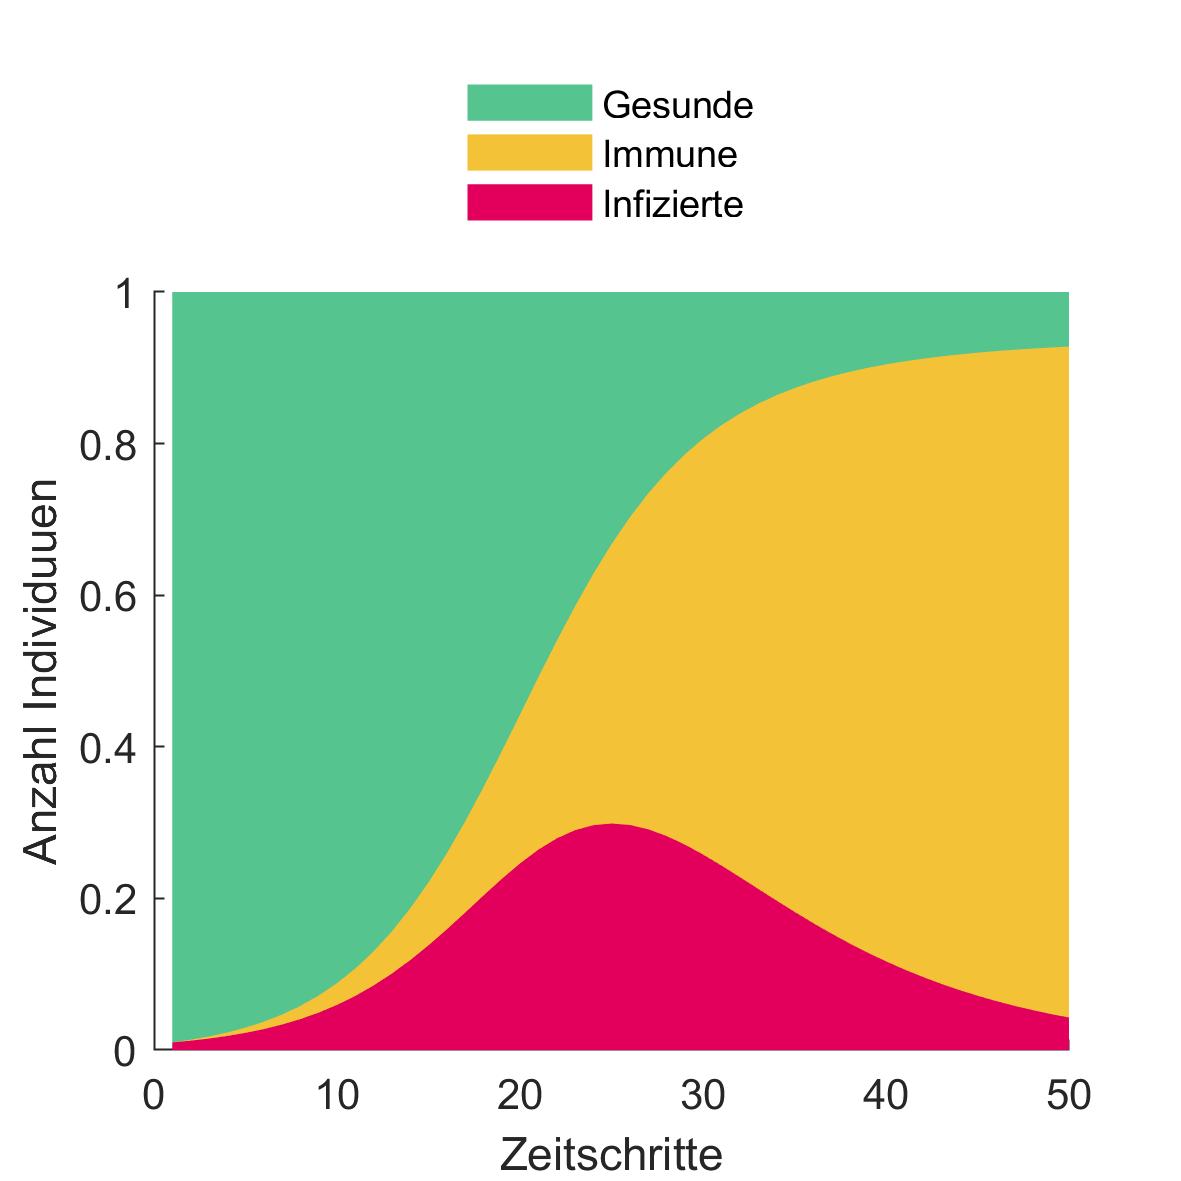
\includegraphics[width=8cm]{SIR.png}
  	\caption{Simulation in MATLAB mit geschätzten Werten (Quelle: Robert Koch Institut) für Covid-19}
  	\begin{align*}
  		\textrm{Basisreproduktionszahl}:\quad
  		R_0 &= \frac{2.4 + 3.3}{2}\\
  		\textrm{Genesungsrate}:\quad
  		\beta &= \frac{1}{8} \quad
  		\textrm{(\textit{Kehrwert ist die Dauer der Infektiosität})}\\
  		\textrm{Infektionsrate}:\quad
  		\alpha &= R_0 \cdot \beta = 0.3562\
  	\end{align*}
\end{figure}


\section{Das SEIR-Modell}
Auch von der Inkubationszeit ist oft die Rede, darum die Erweiterung zum SEIR-Modell. Dabei wird die Gruppe der Infizierten \(I\) aufgeteilt in
\begin{itemize}
	\item \(E_k\): Infizierte Individuen ohne Symptome (Exposed)
Diese Gruppe befindet sich in der Inkubationszeit
	\item \(I_k\): Kranke Individuen (Infected)
Bei diesen Individuen ist die Krankheit ausgebrochen
\end{itemize}
Ich würde die Individuen in der Inkubationszeit auch als ansteckend annehmen. Teilweise wird dies anders gemacht, aber im Falle von Corona scheint es so besser zu passen.
Eigentlich bräuchte es noch eine dritte Gruppe, da ein neu infiziertes Individuum nicht sofort ansteckend ist, aber diese Vereinfachung würde ich hinnehmen.

\noindent
Also sind die Gleichungen mit der Inkubationsrate \(\gamma\) (Kehrwert ist die mittlere Inkubationszeit) neu 
\begin{align*}
	S_{k+1} &= S_k - \alpha \cdot S_k \cdot \left( E_k + I_k \right) \\
	E_{k+1} &= E_k + \alpha \cdot S_k \cdot \left( E_k + I_k \right) - \gamma \cdot E_k \\
	I_{k+1} &= I_k + \gamma \cdot E_k - \beta \cdot I_k \\
	R_{k+1} &= R_k + \beta \cdot I_k
\end{align*}


\begin{figure}[h]
  	\centering
 	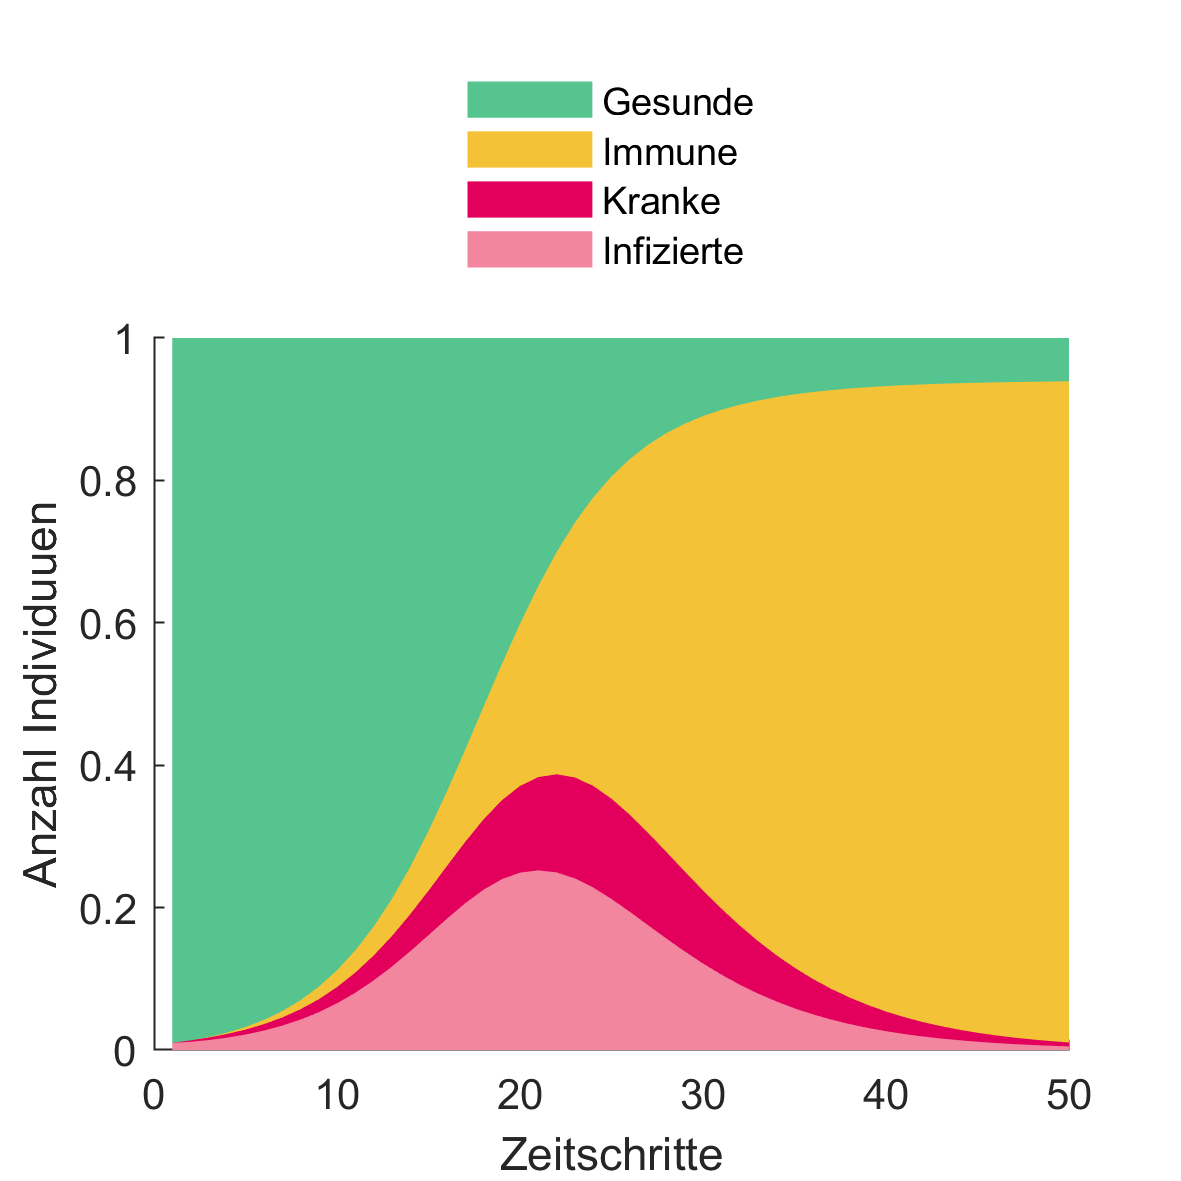
\includegraphics[width=8cm]{SEIR_EplusI.png}
  	\caption{Simulation in MATLAB mit geschätzten Werten (Quelle: Robert Koch Institut) für Covid-19}
  	\begin{align*}
  		\textrm{Basisreproduktionszahl}:\quad
  		R_0 &= \frac{2.4 + 3.3}{2}\\
  		\textrm{Inkubationsrate}:\quad
  		\gamma &= \frac{1}{5} \quad
  		\textrm{(\textit{Kehrwert ist die Inkubationszeit})}\\
  		\textrm{Genesungsrate}:\quad
  		\beta &= \frac{1}{3} \quad
  		\left(\begin{array}{l}
  			\textrm{\textit{Damit gibt sich wiederum eine}}\\
  			\textrm{\textit{Dauer der Infektiosität von 8 Tagen}}
  		\end{array}\right)\\
  		\textrm{Infektionsrate}:\quad
  		\alpha &= R_0 \cdot \frac{1}{8} = 0.3562\
  	\end{align*}
\end{figure}

\newpage

\subsection{Umrechnen in Wahrscheinlichkeiten}
Wie bisher aber halt mit den neuen Gleichungen (\(N\) ist die Gesamtanzahl Individuen)
\begin{align*}
	S_{k+1} &= S_k - S_k \cdot \left( 1 - \left( 1 - a \right)^{\frac{E_k}{N} + \frac{I_k}{N}}\right) \\
	E_{k+1} &= E_k - S_k \cdot \left( 1 - \left( 1 - a \right)^{\frac{E_k}{N} + \frac{I_k}{N}}\right) - c \cdot E_k \\
	I_{k+1} &= I_k + c \cdot E_k - b \cdot I_k \\
	R_{k+1} &= R_k + b \cdot I_k
\end{align*}
\begin{itemize}
	\item Infektionswahrscheinlichkeit \(a\) (\textit{Wiederum über \(R_0\) definiert})
	\item Genesungswahrscheinlichkeit \(b\) (\textit{Kehrwert ist die Zeit vom Ausbruch der Symptome bis zur Genesung})
	\item Wahrscheinlichkeit, dass die Krankheit ausbricht \(c\) (\textit{Kehrwert ist die mittlere Inkubationszeit})
\end{itemize}
\textit{Dieser Teil würde ich unbedingt mit rein nehmen, denn etwas Statistik ist sicher nicht verkehrt.}

\subsection{Vergleich mit einem Zufallsautomaten}
\textit{Dieser Zufallsautomat bedarf sicherlich noch mehr Erklärung, würde aber auch diesen mit rein nehmen, da er doch zeigt, dass der Zufall berechnet werden kann.}
\begin{figure}[h]
  	\centering
 	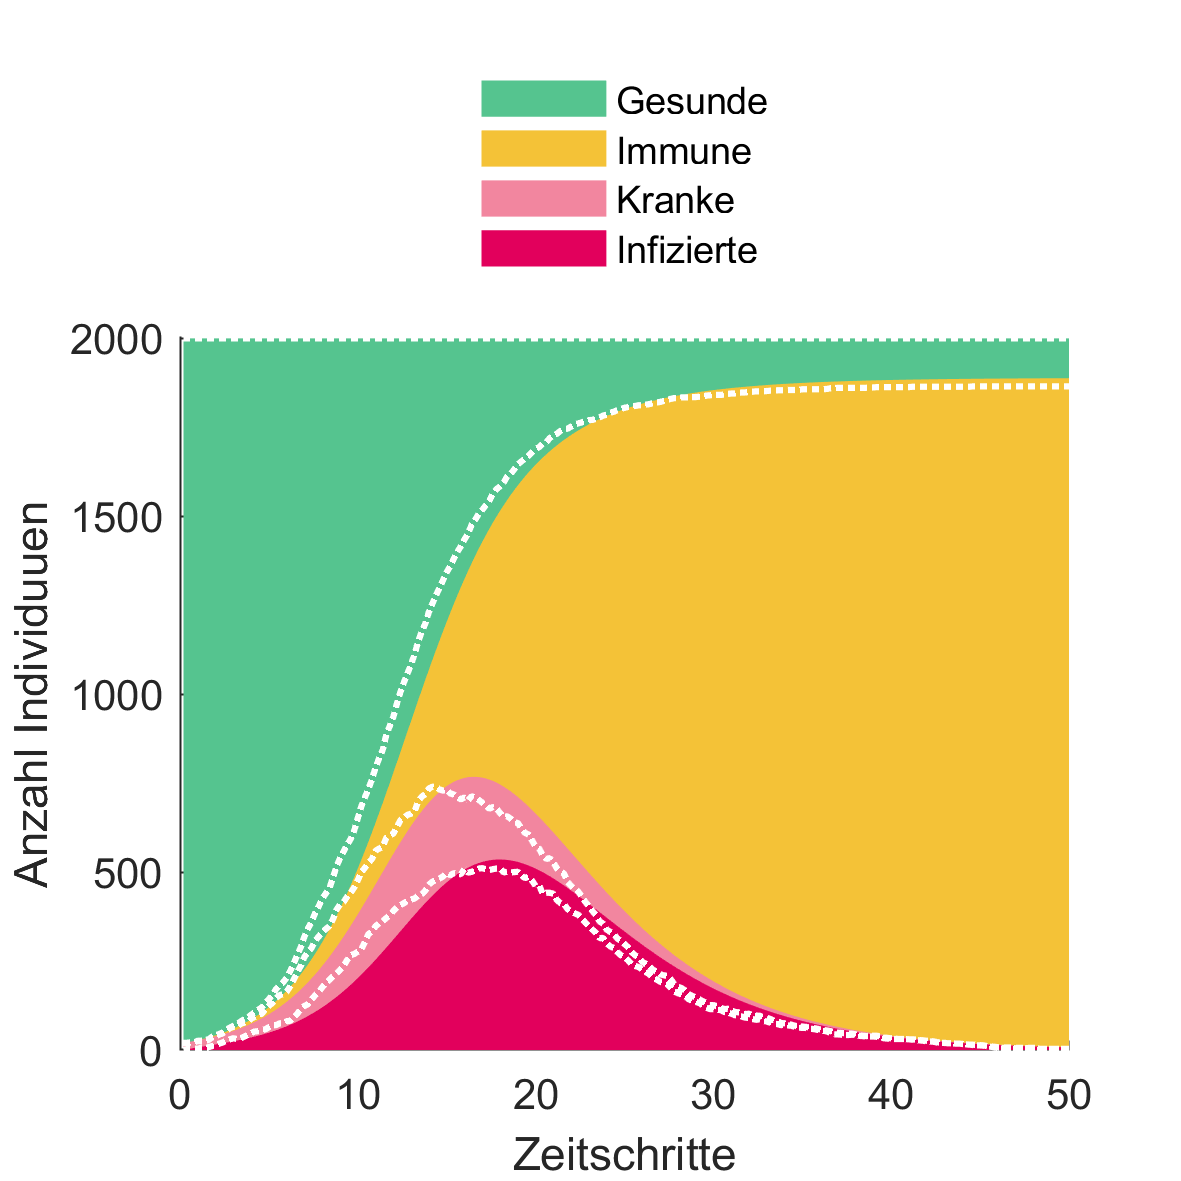
\includegraphics[width=8cm]{diff_vs_randomauto.png}
  	\caption{Simulation des Automaten in MATLAB (gestrichelte Linien) und Vergleich mit den Differenzengleichungen}
  	\begin{align*}
  		\textrm{Größe der Population}:\quad
  		P &= 100'000\\
  		\textrm{Anzahl Zellen}:\quad
  		N &= 200 \cdot 200\\
  		\textrm{Durchschnittliche Anzahl an Kontakten}:\quad
  		k &= \frac{P}{N} = 2.5\\
  		\textrm{Basisreproduktionszahl}:\quad
  		R_0 &= \frac{2.4 + 3.3}{2} = 2.85\\
  		\textrm{W'keit für den Ausbruch}:\quad
  		c &= \frac{1}{5} \quad
  		\textrm{(\textit{Kehrwert ist die Inkubationszeit})}\\
  		\textrm{Genesungsw'keit}:\quad
  		b &= \frac{1}{3}\\
  		\textrm{Dauer der Infektiosität}:\quad
  		D &= \frac{1}{b} + \frac{1}{c}\quad
  		(\textit{Wiederum die 8 Tage})\\
  		\textrm{Infektionsw'keit bei Kontakt}:\quad
  		a &= \frac{R_0}{D \cdot k} = 0.1425\quad
  		\textrm{siehe Quelle bei 2.1}
  	\end{align*}
\end{figure}

\newpage
\section{Der zelluläre Automat}
Die einzelnen Individuen und deren Verhalten muss sehr sehr gut erklärt sein. Ich würde dafür jeweils zu jedem eine kurze Animation mit Text machen. Zusätzlich kommen natürlich die Individuen in der Inkubationszeit dazu und ich würde die Kranken (also da wo die Symptome ausgebrochen sind) nicht mehr bewegen, denn diese liegen ja zuhause im Bett (komplett stillstehen können sie nicht, denn wenn eine Zelle voll wird müssen sie irgendwohin...). Auch sind so milde Verläufe oder Verläufe ohne Symptome nicht berücksichtigt, würde ich aber wiederum auch vernachlässigen.

\textit{Ich würde wiederum etwas Interface machen, damit der Betrachter auch selber damit rumspielen kann. Wobei ich aber nicht die Wahrscheinlichkeiten selber einstellen lassen würde, sondern vielmehr \(R_0\), Inkubationszeit, etc. also die Zahlen die man auch aus der Zeitung kennt. Zusätzlich würde ich jeweils ein Corona Button machen, welcher die geschätzten Werte von der Robert Koch Institut Quelle einstellt.}

\section{Social Distancing}
\textit{bisher Quarantäne Strategien}

\noindent
Die Strategie mit der festen Quarantäne würde ich sicher zeigen, sowie die Strategie mit den Zellen mit Durchgang (evtl. etwas verändert), denn dies ist ja nichts anderes als Social Distancing und das Ergebnis davon ist wie gewünscht flatten the curve.

\section{Deine Strategie}
\textit{Dies war ja schon zu Beginn meine ursprüngliche Idee: Man lässt den Betrachter selber Wände zeichnen. Im Falle von Corona könnte man es sogar so machen, dass er eine Strategie finden muss, dass die Anzahl der Intensivbetten nicht überschritten wird.}



\end{document}